\section{Large Figures}
	\label{sec:app}

\begin{figure}[H] 
	\centering 
	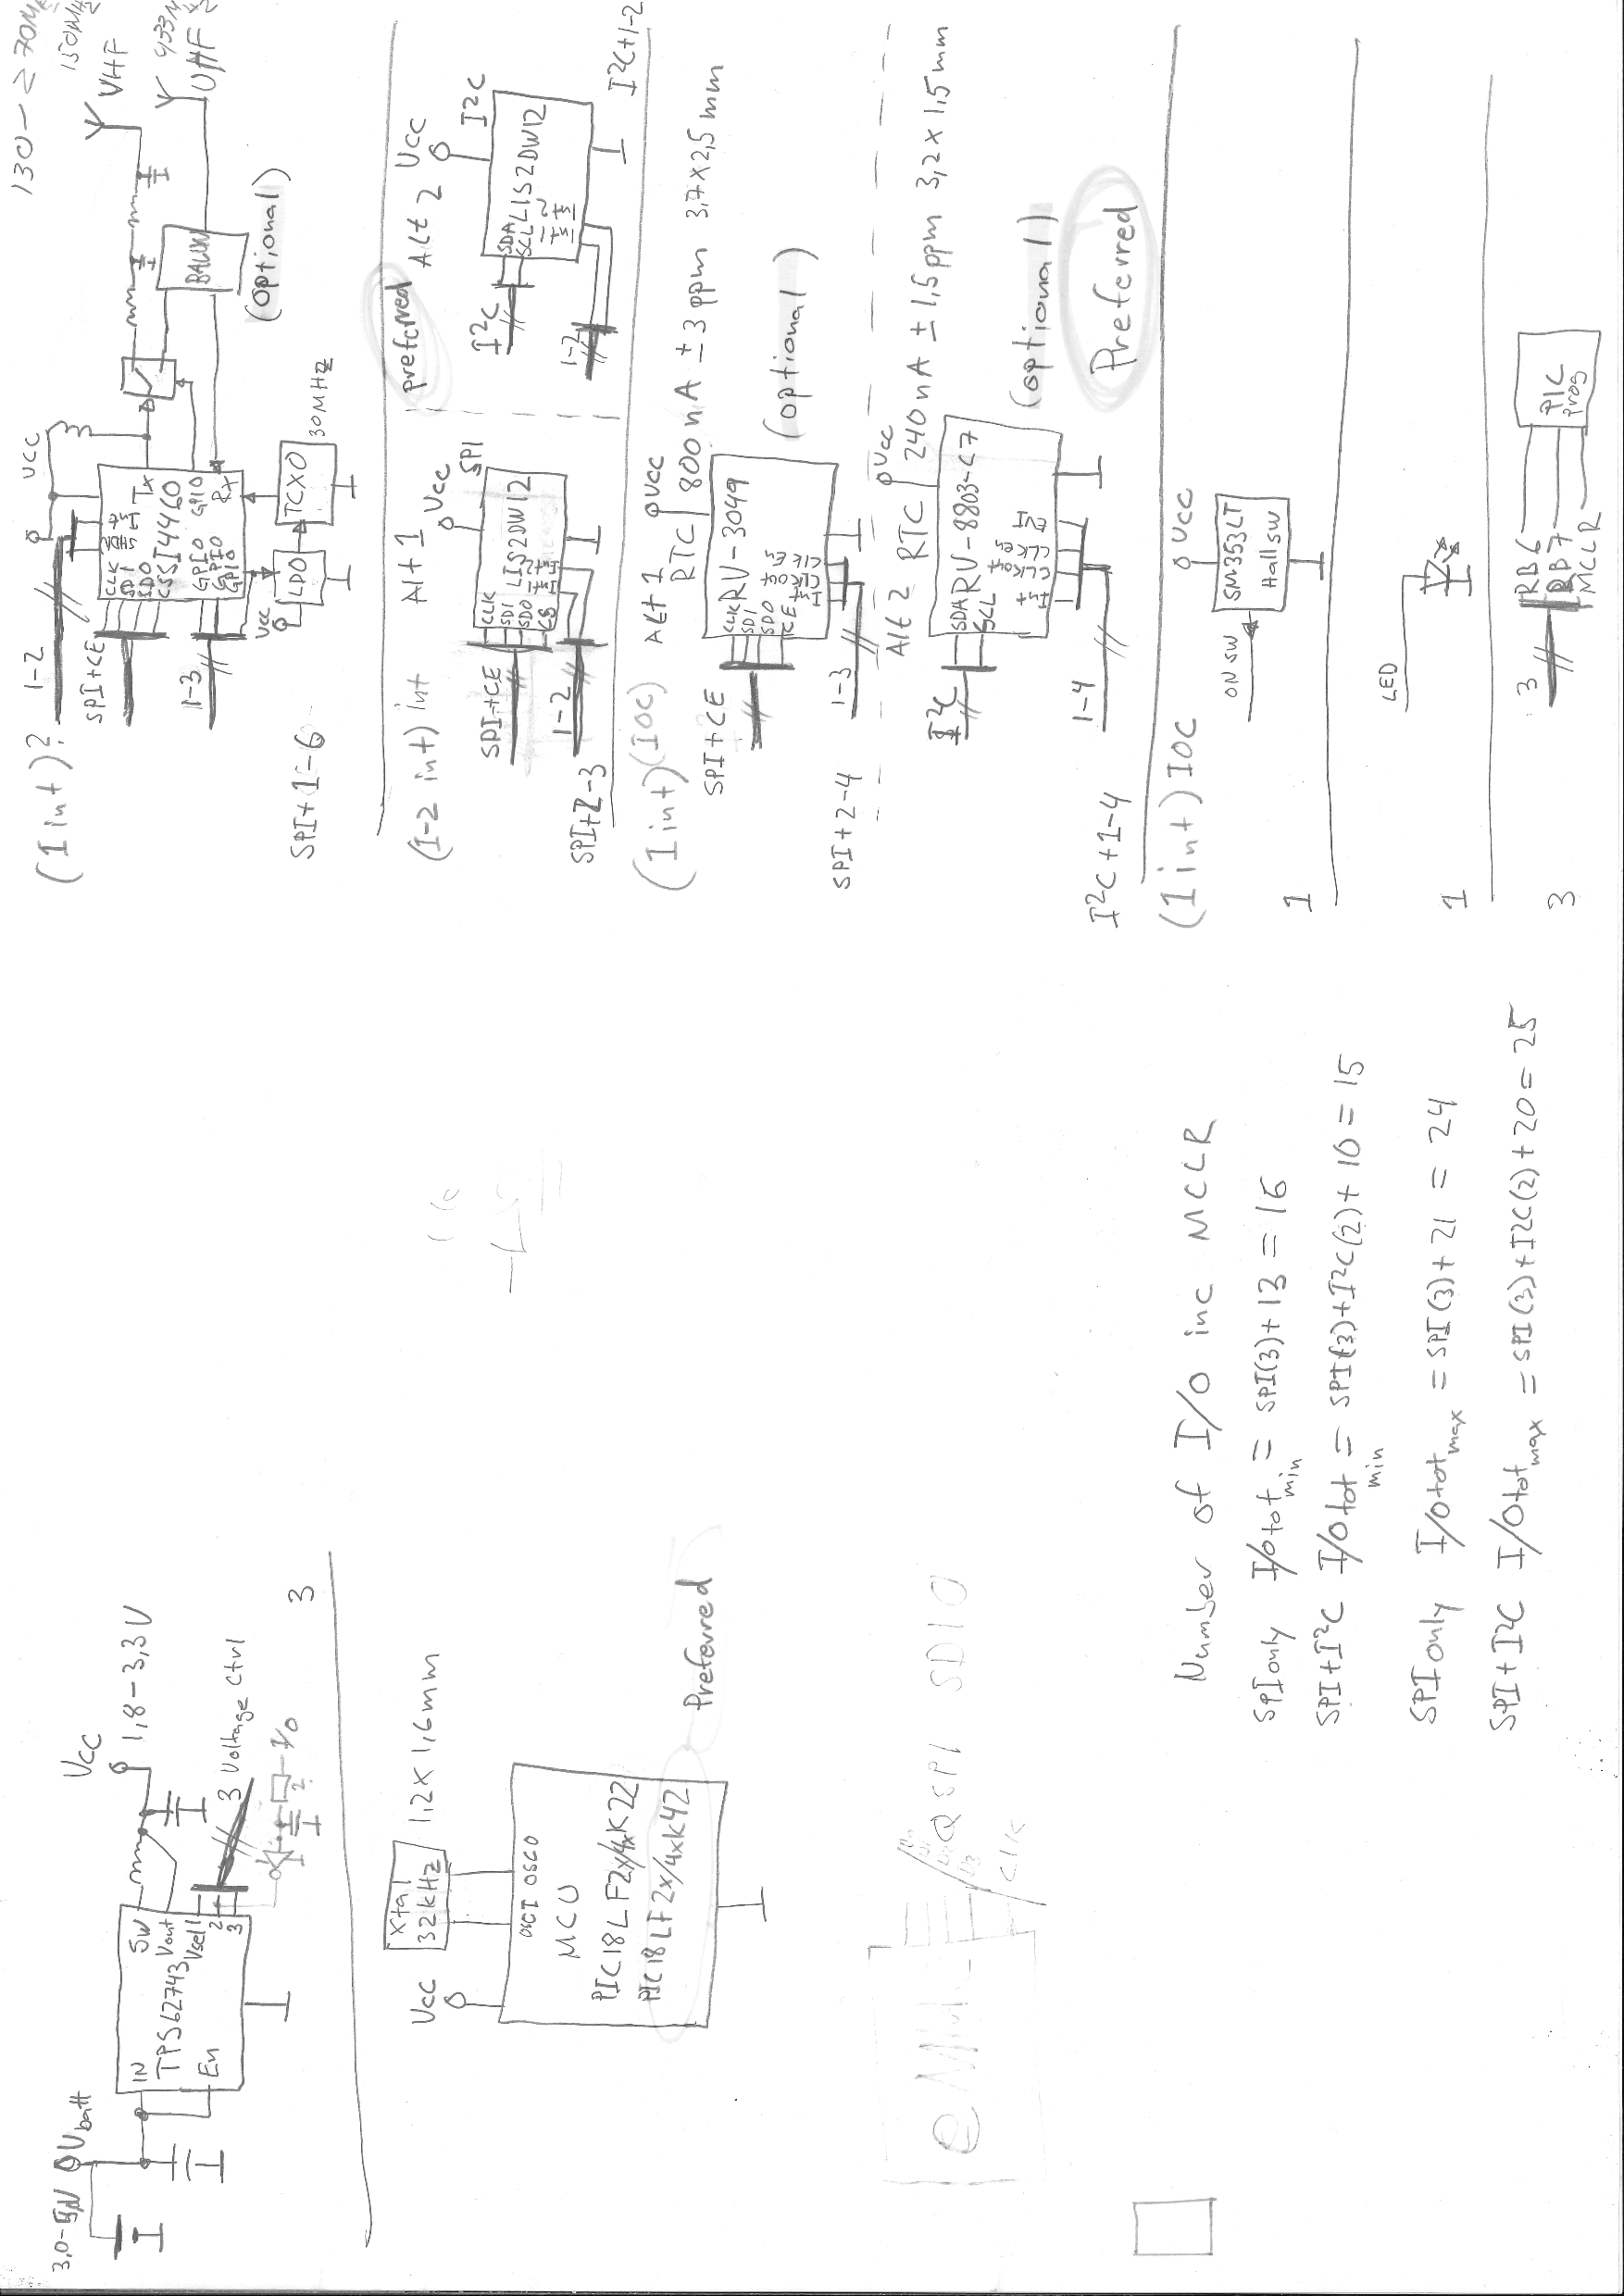
\includegraphics[width=1\linewidth]{Figures/Anders_schema_rot} 
	\captionsource{The initial schematics made by Followit}{Aurthor}
	\label{fig:anders_koppling} 
\end{figure} 

\clearpage
\section{Lists}
\subsection{Bill of Materials: Main \gls{pcb}}
\begin{center}
\begin{tabular}{|l|l|c|}
	\hline
	\bf{Main Board Components} & \bf{Package} & \bf{Quantity} \\
	\hline
	\emph{Capacitors:} & & \\
	\hline
	18p & 0805 & 2 \\
	\hline
	100n & 0805 & 21 \\
	\hline
	1u & 0805 & 2 \\
	\hline 
	2.2u & 0805 & 1 \\
	\hline 
	4.7u & 0805 & 4 \\
	\hline 
	10u & Electrolytic SMD 5x5.3 & 6 \\
	\hline
	\emph{Resistors:} & & \\
	\hline
	220 & 0805 & 1 \\
	\hline
	1k & 0805 & 2 \\
	\hline
	1k & potentiometer & 2 \\
	\hline

\end{tabular}
\end{center}

%\end{center}
%Image of circuit board(s) are sectionlocals labled as "fig:pcbr*"
%Local. Image of casing
%INSERT Image of complete/mounted system